\chapter{User Manuals}

\begin{figure}[h]
\begin{center}
  % Requires \usepackage{graphicx}
  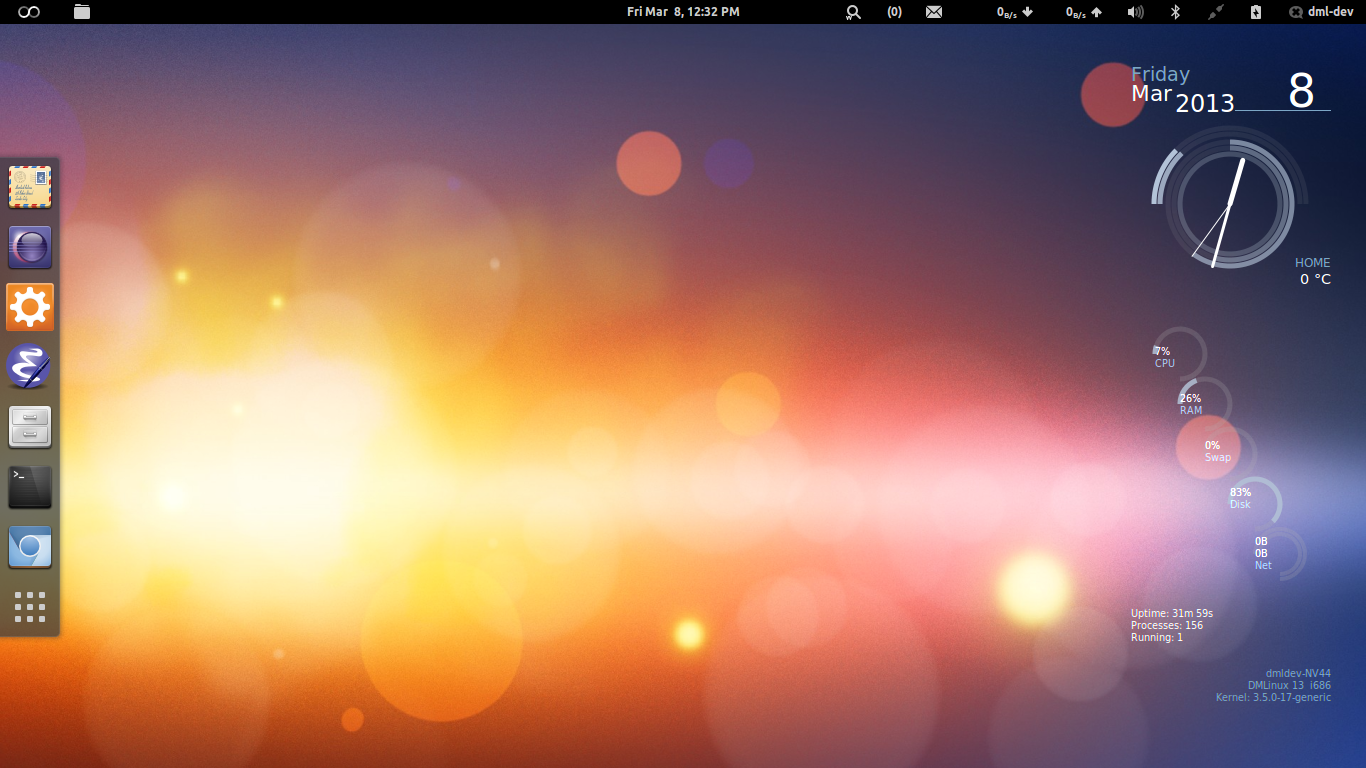
\includegraphics[scale=0.35] {1.png}
  \caption[Screenshot - DMLinux Main Desktop]{Main outlook of DMLinux}
\end{center}
\end{figure}
Description: Above is the Desktop of DMLinux Operating system.It feature GNOME Shell 3.6 inside it.Theme and icons are added by us.

\newpage
\begin{figure}[h]
\begin{center}
  % Requires \usepackage{graphicx}
  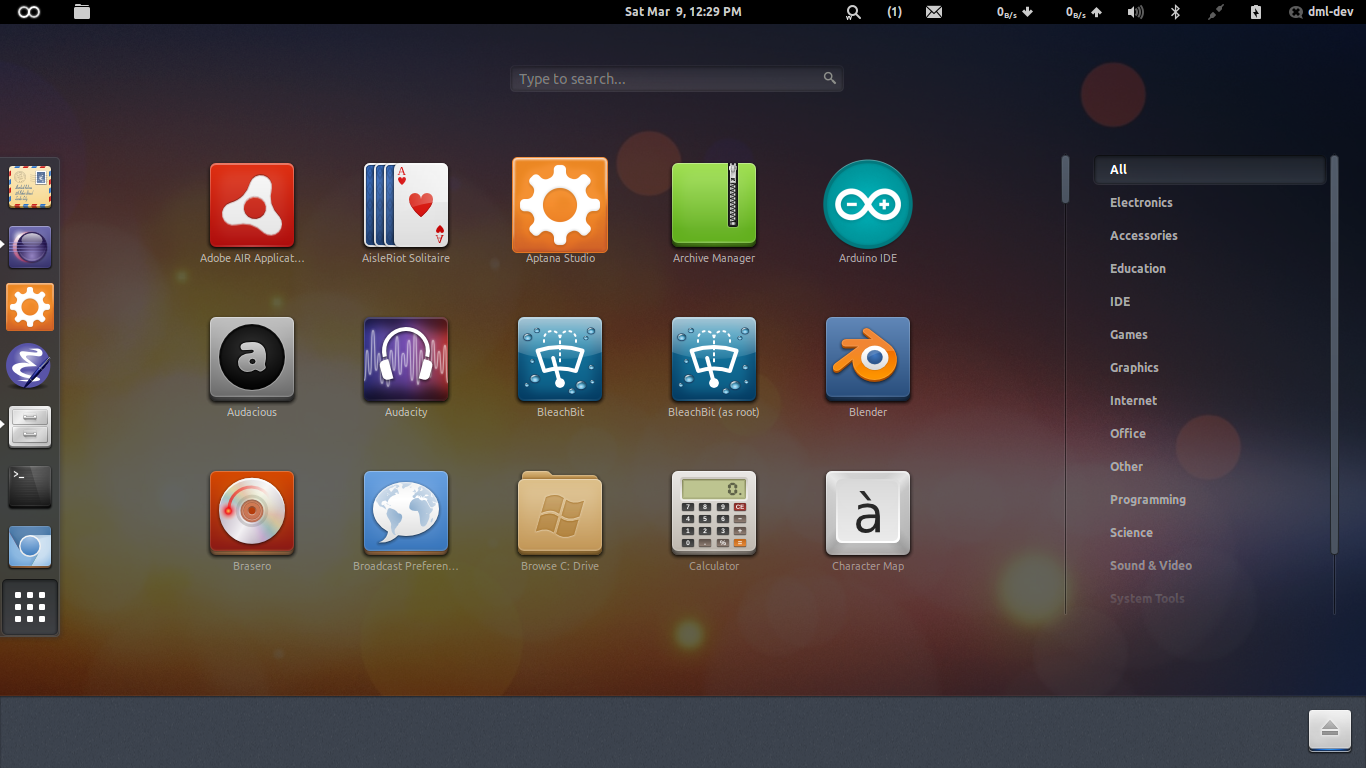
\includegraphics[scale=0.35] {2.png}
  \caption[Screenshot - Application Menu]{Application Menu}
\end{center}
\end{figure}
Description: Above is the screenshot of Application Menu provided in DMLinux .It offeres catogary wise application list.

\newpage
\begin{figure}[h]
\begin{center}
  % Requires \usepackage{graphicx}
  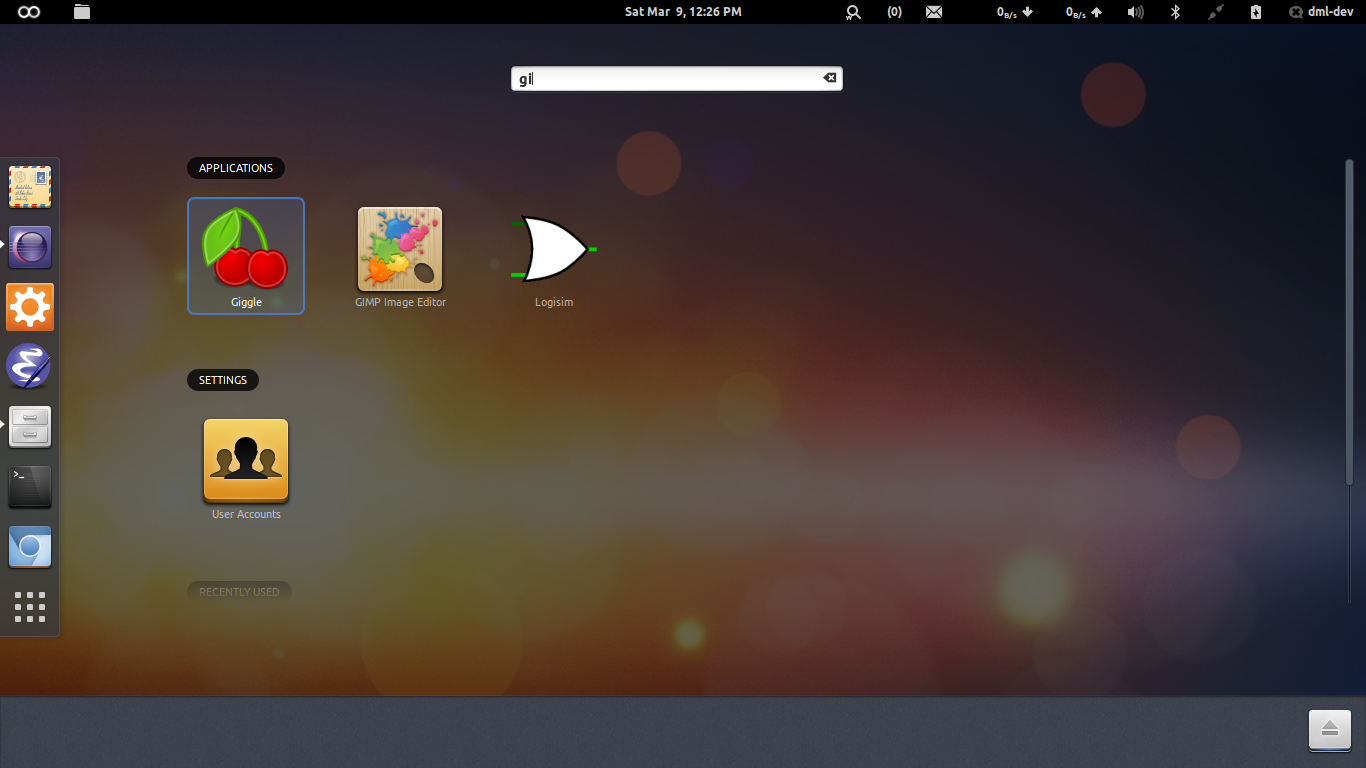
\includegraphics[scale=0.35] {3.png}
  \caption[Screenshot - Search Dash in DMLinux]{Search Dash}
\end{center}
\end{figure}
Description: By pressing Windows Key, User enters in search dash. Here user can search any application,files,settings etc in installed system.

\newpage


\begin{figure}[h]
\begin{center}
  % Requires \usepackage{graphicx}
  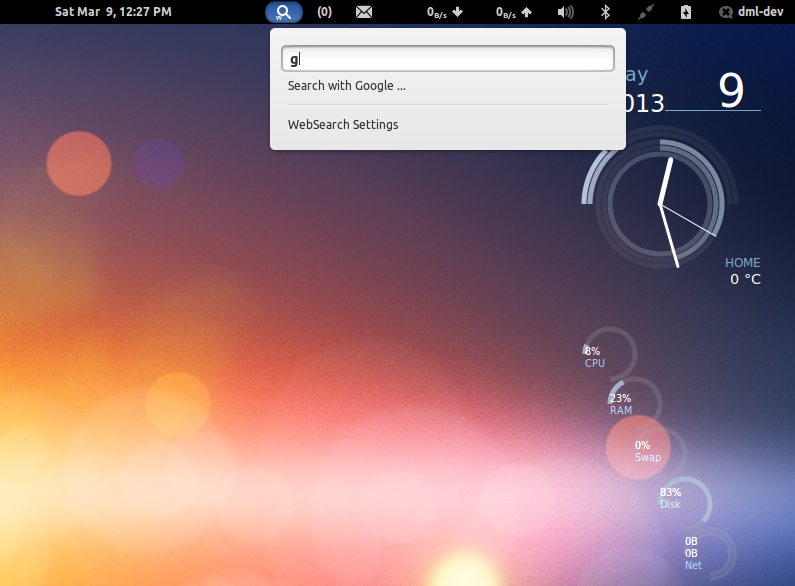
\includegraphics[scale=0.4] {4.png}
  \caption[Screenshot - Web search Applet]{Inbuilt Web Search Applet}
\end{center}
\end{figure}
Description: It is useful applet attached with top panel.User can search on web sites like google and wikipedia directly from here.

\newpage
\begin{figure}[h]
\begin{center}
  % Requires \usepackage{graphicx}
  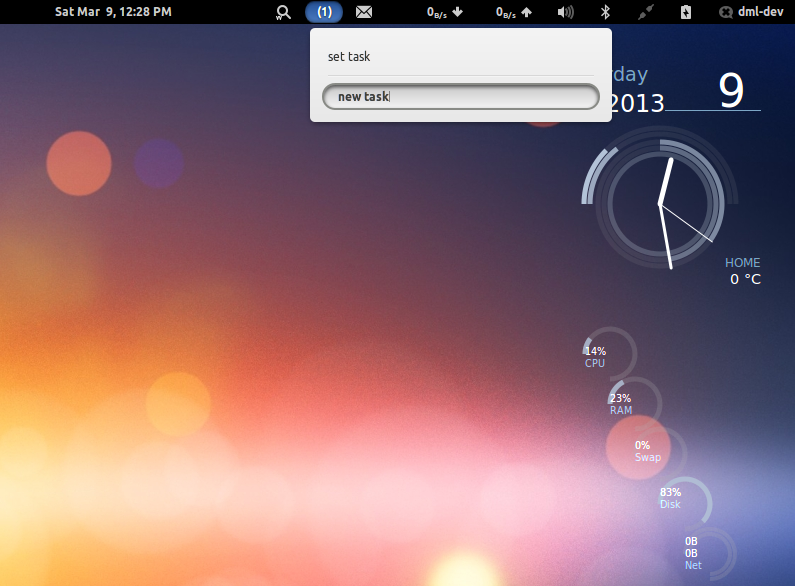
\includegraphics[scale=0.4] {5.png}
  \caption[Screenshot - To-do list applet]{Inbuilt To-do task applet}
\end{center}
\end{figure}
Description: It is useful applet attached with top panel.User can make to-do list of everday' task and whenever its completed,he/she can delete it by clicking on that task.
\newpage
\begin{figure}[h]
\begin{center}
  % Requires \usepackage{graphicx}
  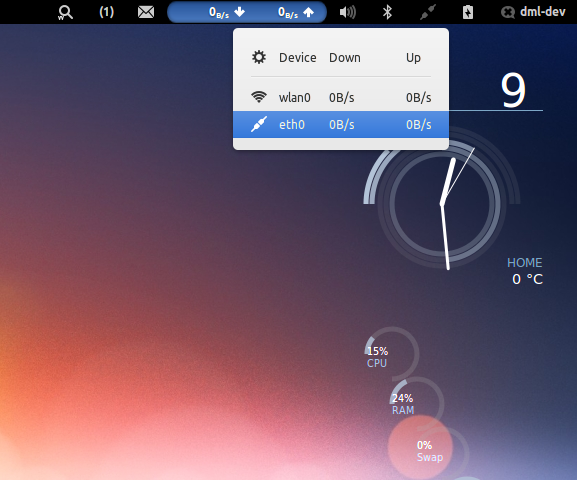
\includegraphics[scale=0.4] {6.png}
  \caption[Screenshot - Network Meter]{Network Meter}
\end{center}
\end{figure}
Description: It is a live network monitor attached with top panel.User can see the speed of network via this applet.

\newpage
\begin{figure}[h]
\begin{center}
  % Requires \usepackage{graphicx}
  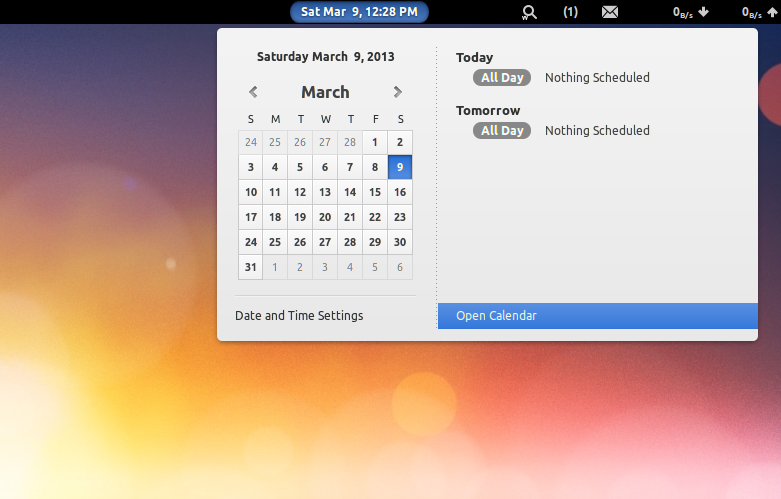
\includegraphics[scale=0.4] {7.png}
  \caption[Screenshot - Calender applet]{Calendar support}
\end{center}
\end{figure}
Description: Above feature is useful to plan a task or month using calendar on Evolution Mail client.It is handy tool with top panel for plainnig big task or any important task.

\newpage

\begin{figure}[h]
\begin{center}
  % Requires \usepackage{graphicx}
  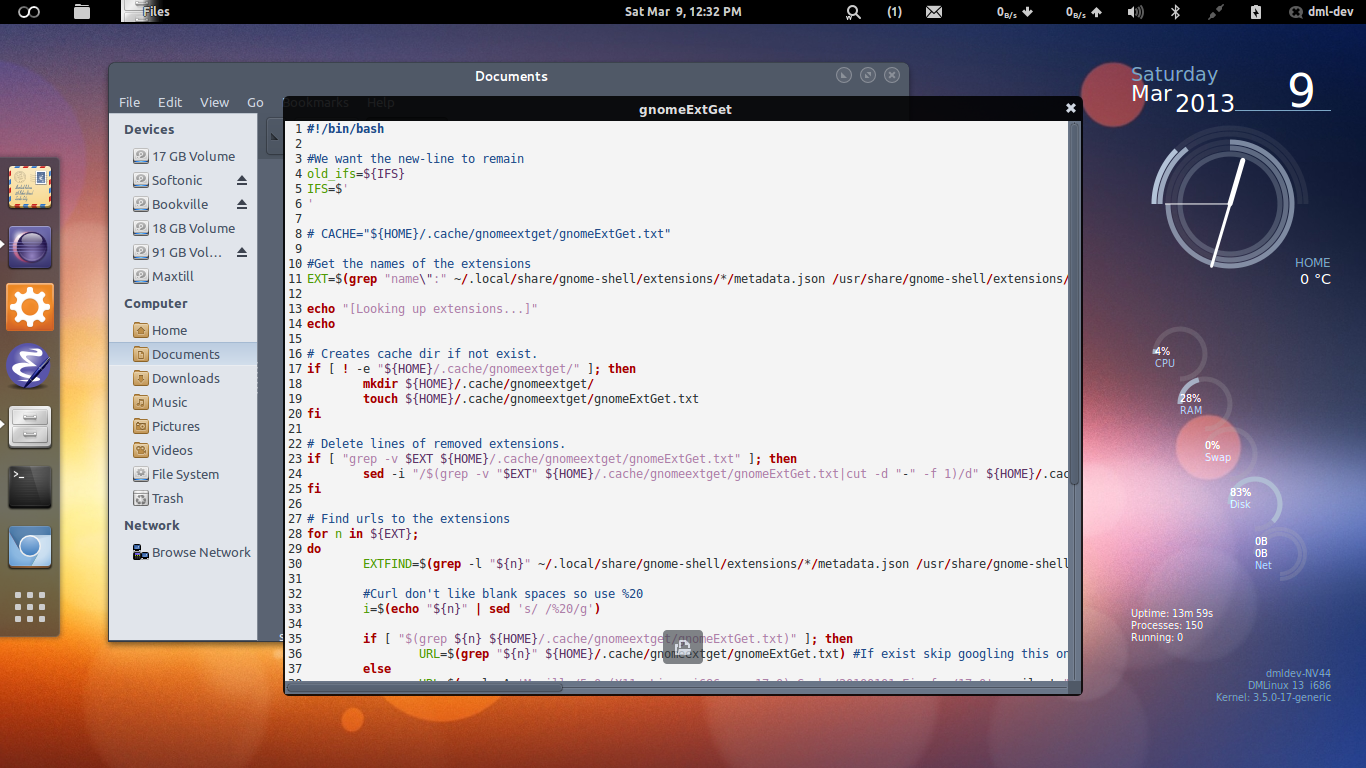
\includegraphics[scale=0.35] {8.png}
  \caption[Screenshot - Quick Preview]{Quick Preview support}
\end{center}
\end{figure}
Description: User can see the preview of txt,folders,pdf,image,music and video files directly by pressing SPACE BAR on the file in file manager.It is useful feature of GNOME Shell 3.6.
\newpage
\begin{figure}[h]
\begin{center}
  % Requires \usepackage{graphicx}
  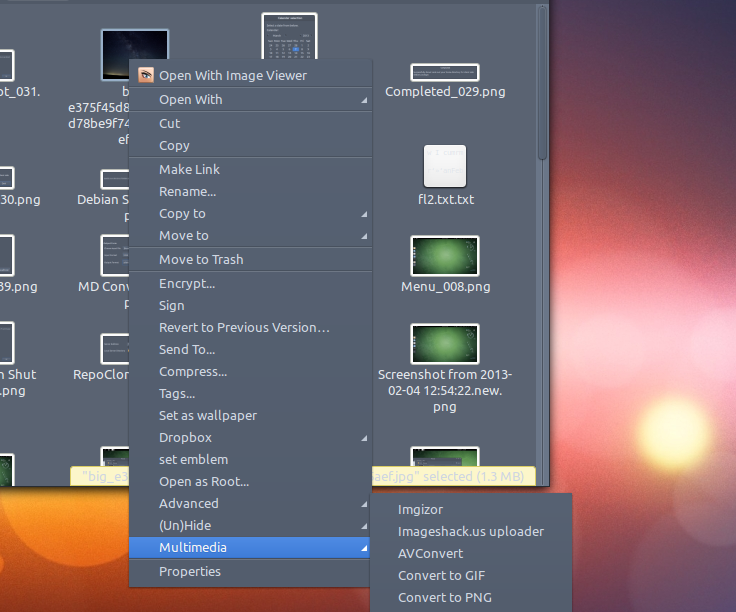
\includegraphics[scale=0.4] {9.png}
  \caption[Screenshot - Extended Right Menu]{Extended right menu}
\end{center}
\end{figure}
Description : Extended right menu provides lots of feature that can be directly performed on file or folder via clicking right mouse button.It has handsfull features like image resizing,hide/unhide,checksum,dropbox sharing etc.It is nautilus extra package provided in the system.
\newpage
\begin{figure}[h]
\begin{center}
  % Requires \usepackage{graphicx}
  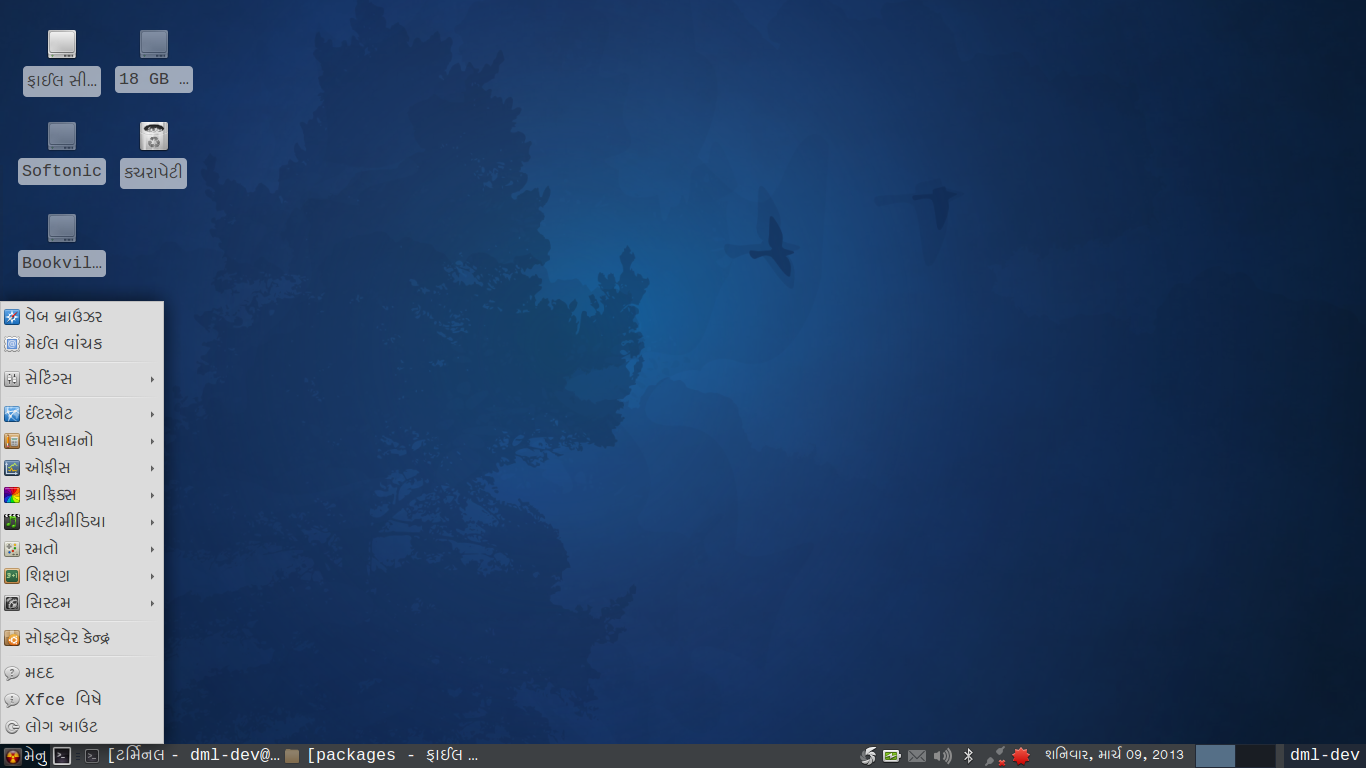
\includegraphics[scale=0.35] {10.png}
  \caption[Screenshot - OpenGujarat Main Desktop]{OpenGujarat Main Desktop View}
\end{center}
\end{figure}
Description: This is a screenshot of OpenGujarat OS Main Desktop View.It contains XFCE 4.1 Desktop Environment.It is designed as windows type mock up by us.
\newpage


\begin{figure}[h]
\begin{center}
  % Requires \usepackage{graphicx}
  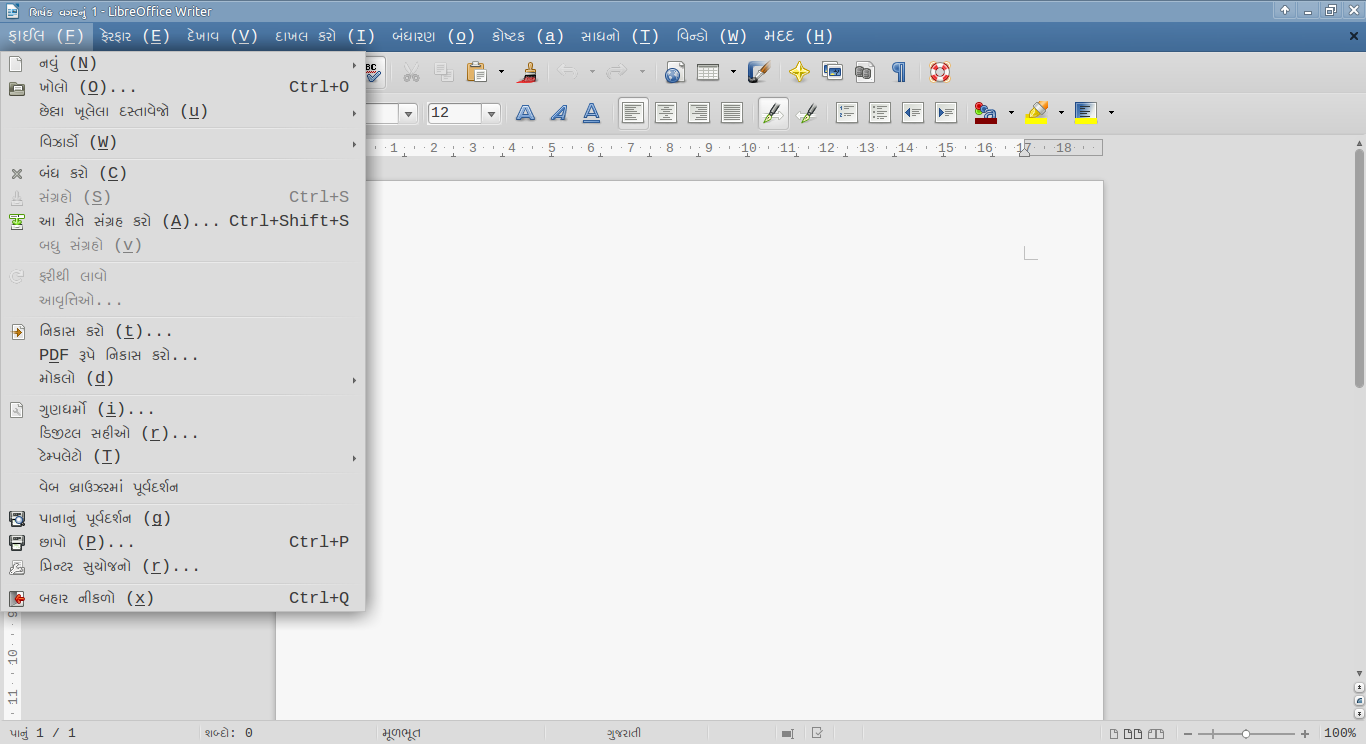
\includegraphics[scale=0.35] {11.png}
  \caption[Screenshot - Office suite in Gujarati]{LibreOffice suite in Gujarati}
\end{center}
\end{figure}
Description: Above is screenshot of LibreOffice suite inbuilt in OpenGujarat OS.

\newpage
\begin{figure}[h]
\begin{center}
  % Requires \usepackage{graphicx}
  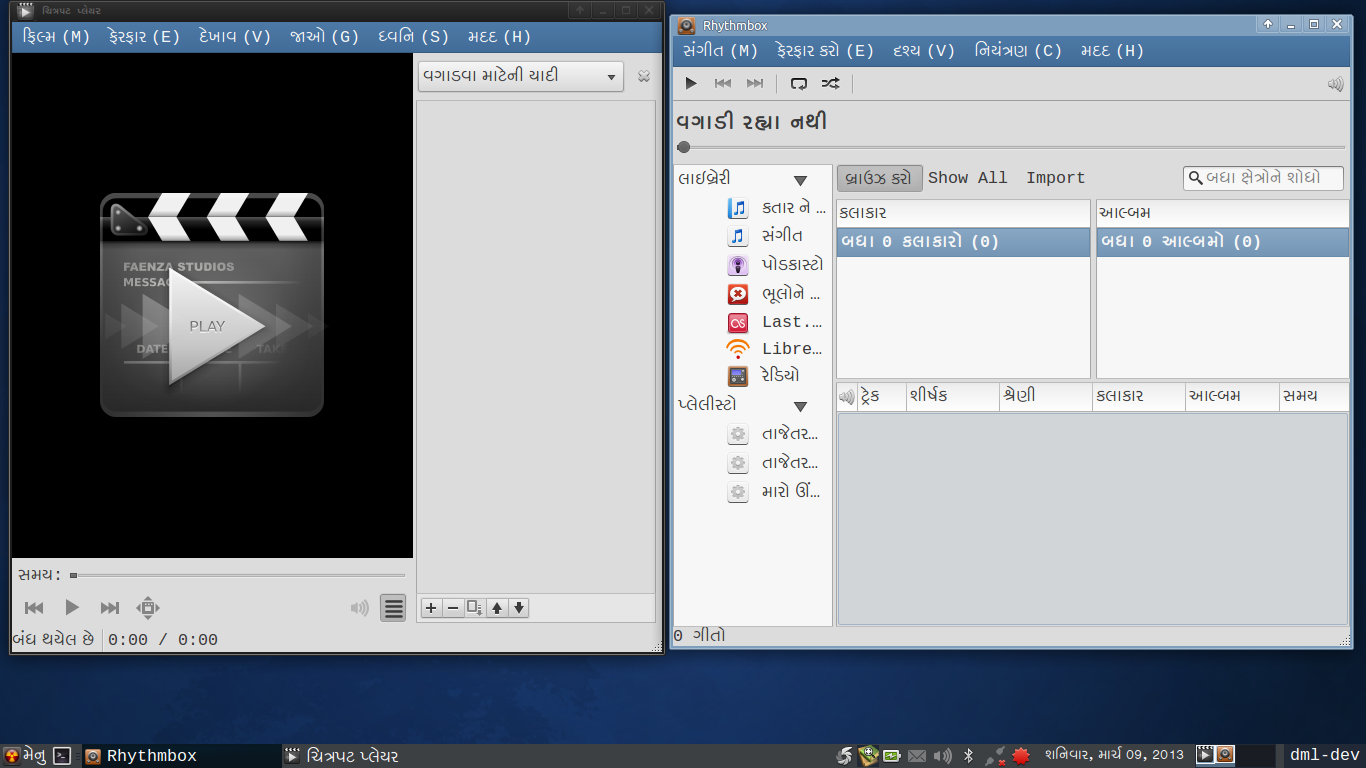
\includegraphics[scale=0.35] {12.png}
  \caption[Screenshot - Music and Media player in OpenGujarat]{Music and Media Player in Gujarati}
\end{center}
\end{figure}
Description:  Above is screenshot of Music and Media player inbuilt in OpenGujarat OS.

\newpage

\begin{figure}[h]
\begin{center}
  % Requires \usepackage{graphicx}
  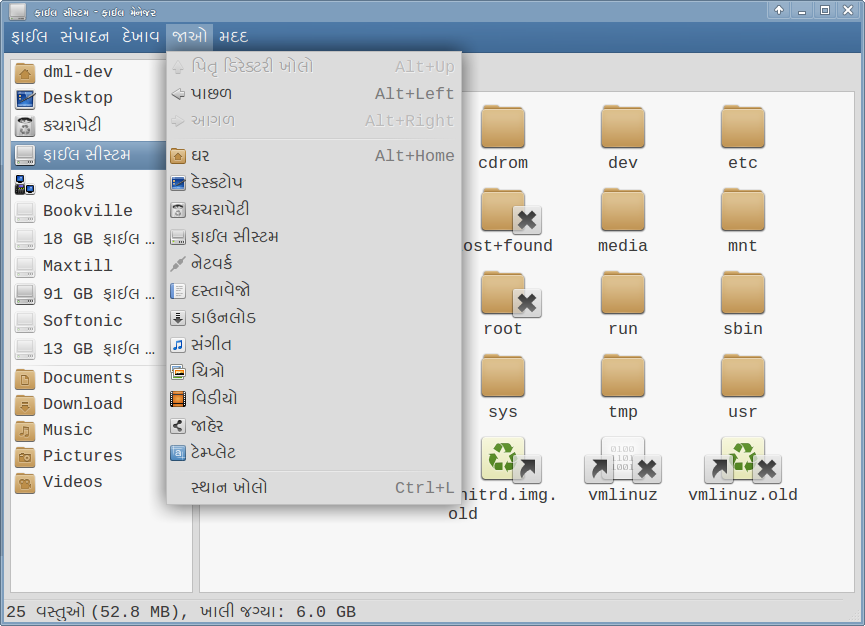
\includegraphics[scale=0.4] {13.png}
 \caption[Screenshot - Thunar File manager]{Thunar File manager}
\end{center}
\end{figure}
Description: It is screenshot of thunar file manager translated in gujarati provided in OpenGujarat.

\newpage
\begin{figure}[h]
\begin{center}
  % Requires \usepackage{graphicx}
  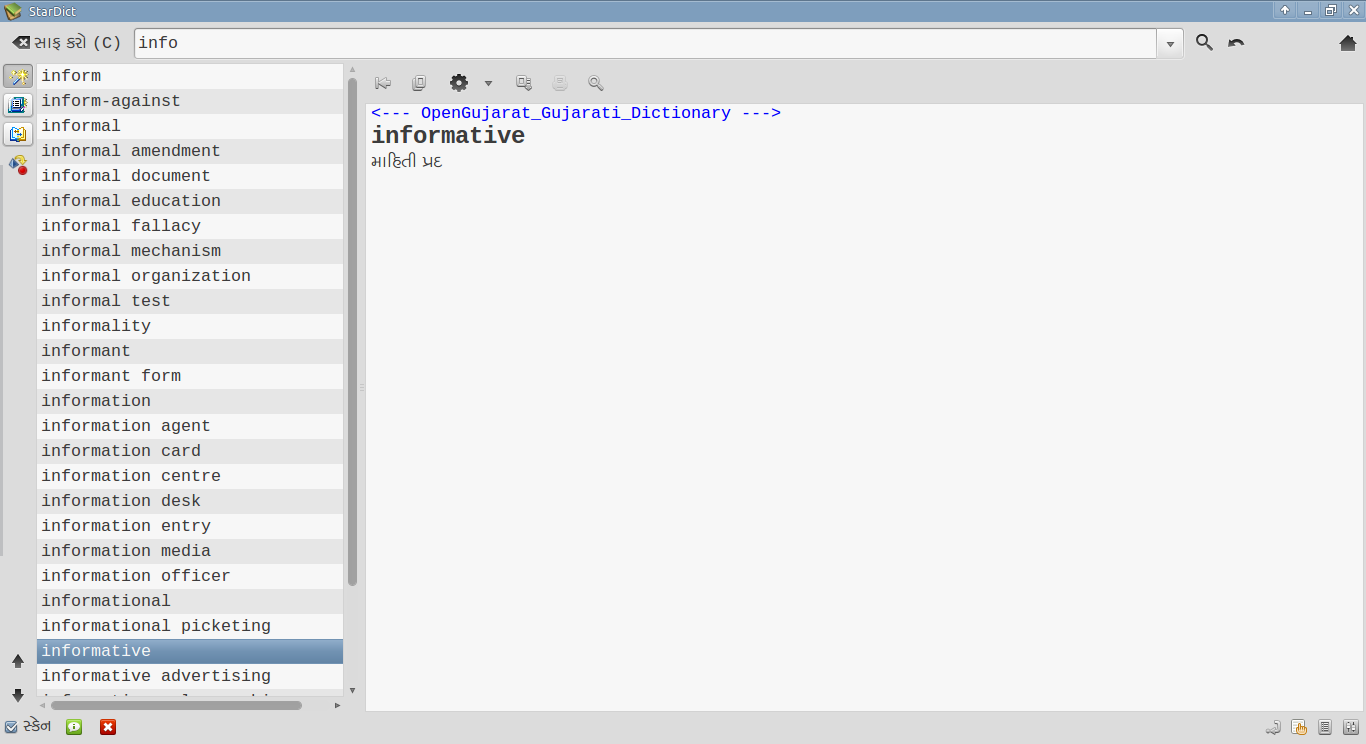
\includegraphics[scale=0.4] {14.png}
  \caption[Screenshot - Gujarati Dictionary]{Gujarati Dictionary Main View}
\end{center}
\end{figure}
Description: It is main search bar of Gujarati dictionary with stardict dictionary look up program.
\newpage

\begin{figure}[h]
\begin{center}
  % Requires \usepackage{graphicx}
  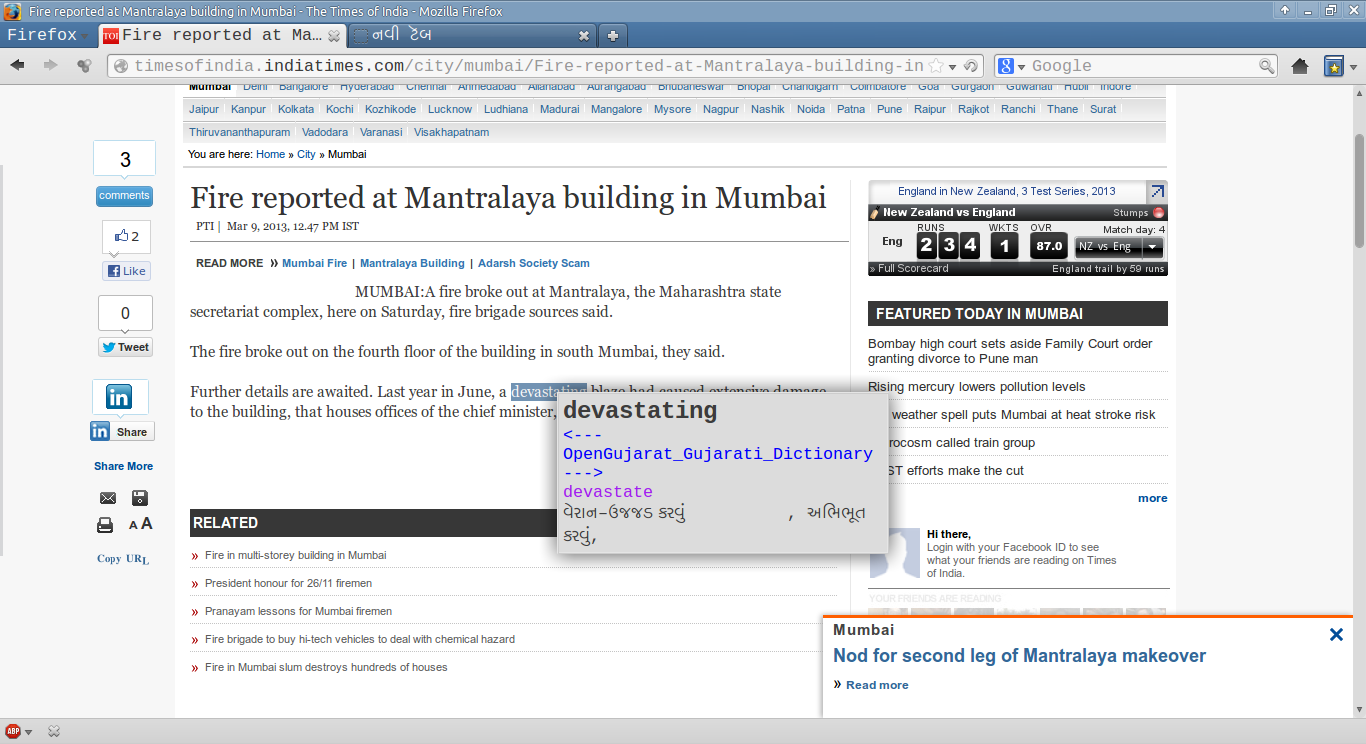
\includegraphics[scale=0.35] {15.png}
  \caption[Screenshot - Gujarati Dictionary Live search]{Gujarati Dictionary Live search}
\end{center}
\end{figure}
Description: Here is the output as dialog box clicked on the word to get the meaning of English word in Gujarati dictionary.Result is provided by Stardict application as pop up box.

\newpage
\begin{figure}[h]
\begin{center}
  % Requires \usepackage{graphicx}
  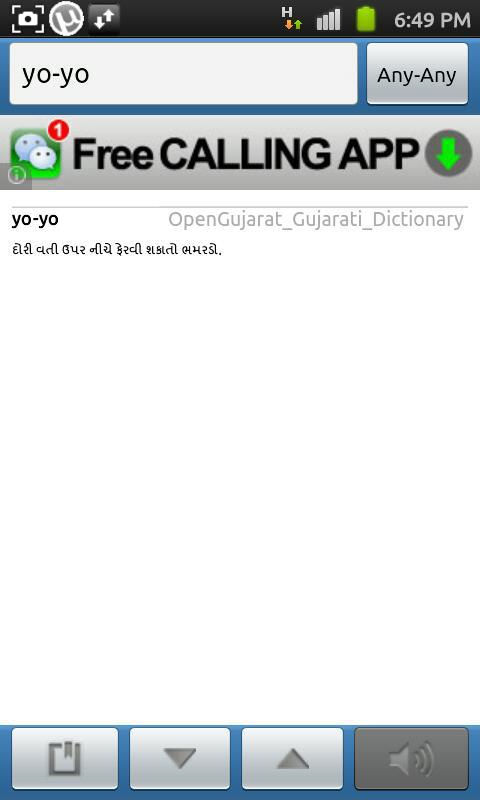
\includegraphics[scale=0.67] {16.png}
  \caption[Screenshot - Gujarati Dictionary Android View]{Gujarati Dictionary Android View}
\end{center}
\end{figure}
Description: It is a screenshot of Gujarati dictionary ported to android phone via GoldenDict Dictionary Look up program.
\newpage
\begin{figure}[h]
\begin{center}
  % Requires \usepackage{graphicx}
  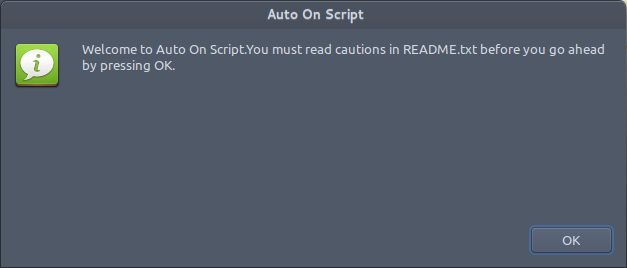
\includegraphics[scale=0.65] {17.png}
  \caption[Screenshot - Auto ON Utility Start Up screen]{Auto ON Utility Start Up screen}
\end{center}
\end{figure}
Description: Here is the start up screen of auto on utility .
\begin{figure}[h]
\begin{center}
  % Requires \usepackage{graphicx}
  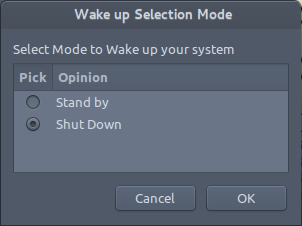
\includegraphics[scale=0.79] {18.png}
  \caption[Screenshot - Mode selection in Auto ON Utility]{Mode selection in Auto ON Utility}
\end{center}
\end{figure}
Description: User have to select in which mode he/she wants to boot pc after given time.

\begin{figure}[h]
\begin{center}
  % Requires \usepackage{graphicx}
  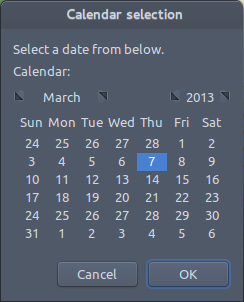
\includegraphics[scale=0.79] {19.png}
  \caption[Screenshot - Date Selection]{Date selection}
\end{center}
\end{figure}

\begin{figure}[h]
\begin{center}
  % Requires \usepackage{graphicx}
  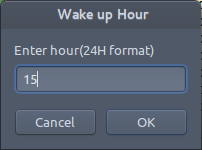
\includegraphics[scale=0.99] {20.png}
  \caption[Screenshot - Hour Entry Box]{Hour Entry Box}
\end{center}
\end{figure}
\begin{figure}[h]
\begin{center}
  % Requires \usepackage{graphicx}
  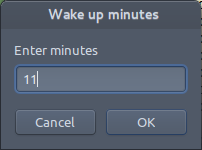
\includegraphics[scale=0.99] {21.png}
  \caption[Screenshot - Minutes Entry Box]{Minutes Entry Box}
\end{center}
\end{figure}\begin{figure}[h]
\begin{center}
  % Requires \usepackage{graphicx}
  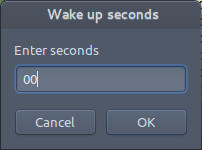
\includegraphics[scale=0.99] {22.png}
  \caption[Screenshot - Seconds Entry Box]{Seconds Entry Box}
\end{center}
\end{figure}

\begin{figure}[h]
\begin{center}
  % Requires \usepackage{graphicx}
  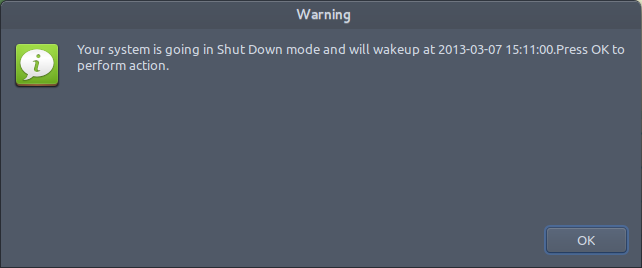
\includegraphics[scale=0.69] {23.png}
  \caption[Screenshot - Final warning of Auto ON Utility]{Final warning of Auto ON Utility}
\end{center}
\end{figure}

\begin{figure}[h]
\begin{center}
  % Requires \usepackage{graphicx}
  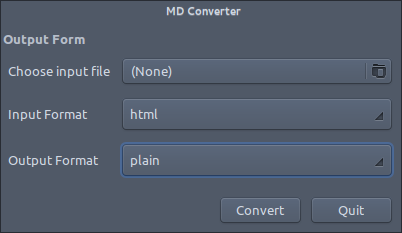
\includegraphics[scale=0.89] {24.png}
  \caption[Screenshot - MDConverter Main Screen]{Main Screen of MDCoverter}
\end{center}
\end{figure}
\begin{figure}[h]
\begin{center}
  % Requires \usepackage{graphicx}
  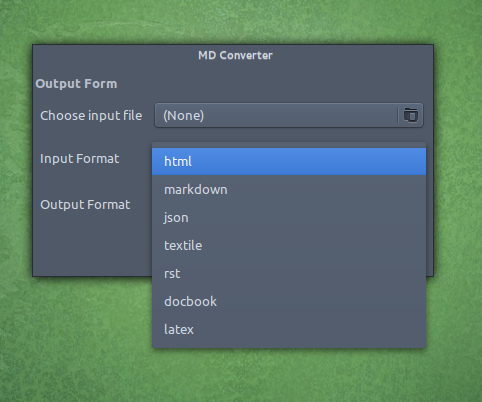
\includegraphics[scale=0.89] {25.png}
  \caption[Screenshot - MDConverter Input Options]{MDConverter Input Options}
\end{center}
\end{figure}
\begin{figure}[h]
\begin{center}
  % Requires \usepackage{graphicx}
  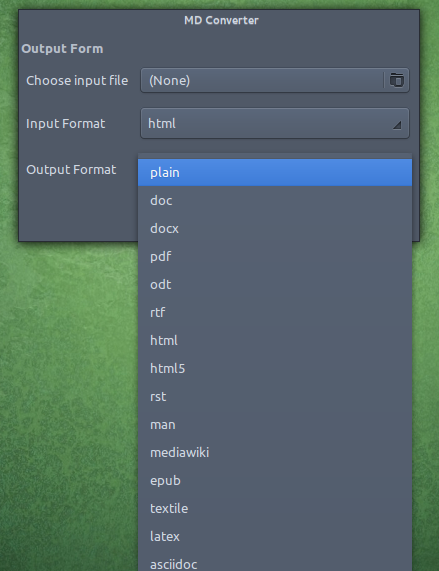
\includegraphics[scale=0.89] {26.png}
  \caption[Screenshot - MDConverter Output Options]{MDConverter Output Options}
\end{center}
\end{figure}
\newpage
\begin{figure}[h]
\begin{center}
  % Requires \usepackage{graphicx}
  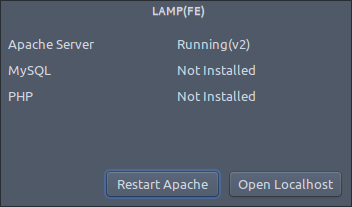
\includegraphics[scale=0.89] {27.png}
  \caption[Screenshot - LAMP Front End]{LAMP Front end Main Screen}
\end{center}
\end{figure}
\begin{figure}[h]
\begin{center}
  % Requires \usepackage{graphicx}
  
\includegraphics[scale=0.69] {28.png}
  \caption[Screenshot - LAMP Apache Server Restart Notification]{LAMP Apache Server Restart Notification}
\end{center}
\end{figure}
\newpage
\begin{figure}[h]
\begin{center}
  % Requires \usepackage{graphicx}
  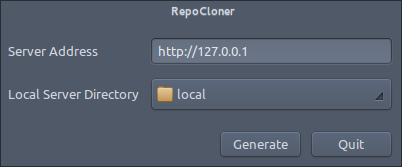
\includegraphics[scale=0.89] {29.png}
  \caption[Screenshot - Repocloner Front End]{Repocloner Front End}
\end{center}
\end{figure}
\begin{figure}[h]
\begin{center}
  % Requires \usepackage{graphicx}
  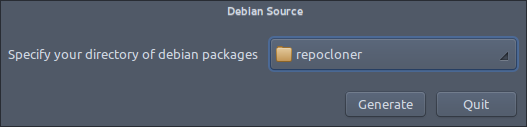
\includegraphics[scale=0.89] {30.png}
  \caption[Screenshot - Repocloner Debian Source Dialog box]{Repocloner Debian Source Dialog box}
\end{center}
\end{figure}\begin{figure}[h]
\begin{center}
  % Requires \usepackage{graphicx}
  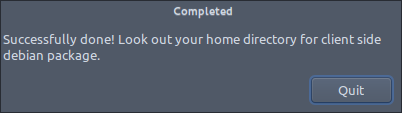
\includegraphics[scale=0.89] {31.png}
  \caption[Screenshot - Repocloner Final Dialog]{Repocloner Final Dialog}
\end{center}
\end{figure}
